%% Report on the S3-3HDM scalar sector in the soft-broken vacuum.
%% Companion: derivations_05.tex (the derivation ledger, auto-generated by the notebook).
%% Source: research/thdm_s3/05_soft_scalar_scan.ipynb
\documentclass[11pt,a4paper]{article}
\usepackage[T1]{fontenc}
\usepackage[utf8]{inputenc}
\usepackage{amsmath,amssymb}
\usepackage{graphicx}
\usepackage{booktabs}
\usepackage[margin=2.4cm]{geometry}
\usepackage[colorlinks=true,linkcolor=blue,citecolor=blue,urlcolor=blue]{hyperref}
\setlength{\parindent}{0pt}
\setlength{\parskip}{0.6em}

\title{The $S_3$-symmetric 3HDM in the soft-broken vacuum:\\
a decoupling-like spectrum, and why the light scalars\\
of the exact-$S_3$ scan do not survive}
\author{M. Zeleny-Mora\\[2pt]
\small Instituto de Física, Universidad Nacional Autónoma de México}
\date{\today}

\begin{document}
\maketitle

\begin{abstract}
\noindent
The exact-$S_3$ potential forces the vacuum onto the $\sqrt3$ alignment. That alignment
forces $V_{us}=0$, and soft $S_3$ breaking is what lifts it (companion fermion report). I
have re-run the full scalar parameter scan in the soft-broken vacuum, with the same theory
and collider cuts, over a 13-dimensional space: eight quartics, two vacuum angles and three
free soft masses. 2021 of $1.1\times10^8$ sampled points survive. The spectrum changes
character. The SM-like state is the lightest CP-even scalar in 99.7\% of points, the heavy
states are near-degenerate and reach the TeV scale, and the light scalars that 16\% of the
exact-$S_3$ points carry drop to 0.7\%. Those light states are a property of the
measure-zero exact slice, not of the $S_3$ quartics. Along the way, two structural results
fix how the scan has to be set up: a coordinate pole in the natural parametrisation of the
tadpoles, and a fundamental domain for the vacuum angle.
\end{abstract}

\section{Summary}

Everything below comes from \texttt{research/thdm\_s3/05\_soft\_scalar\_scan.ipynb}; the
scan itself is \texttt{scan\_soft.py}, and its output is
\texttt{results/viable\_points\_soft.json}.

\begin{enumerate}\itemsep2pt
\item \textbf{Soft does not mean small} (\S\ref{sec:soft}). The soft terms are sampled
wide, and how close a point is to exact $S_3$ is read off afterwards instead of being
imposed.
\item \textbf{A parametrisation pole, avoided}: solving the tadpoles for the wrong soft term
divides by $v_1^2-v_2^2$ (\S\ref{sec:tadpoles}).
\item \textbf{$\varphi\in(0,\pi/3)$ is a fundamental domain}, and our quark-fit vacuum sits
inside it at $\varphi=53.4^\circ$ (\S\ref{sec:domain}).
\item \textbf{The spectrum machinery generalises}: the Goldstones stay isolated, and the
CP-even sector becomes a full $3\times3$ with no gauge-phobic state (\S\ref{sec:spectrum}).
\item \textbf{The soft-broken spectrum is decoupling-like}, and the exact scan's light
scalars do not survive generic soft breaking (\S\ref{sec:results}). This is the main
result.
\end{enumerate}

\section{What ``soft'' means}
\label{sec:soft}

The soft-broken potential adds the four CP-conserving, gauge-invariant quadratics that break
$S_3$:
\[
V_{\rm soft}=m_{D1}^2(x_{11}-x_{22})-m_{D2}^2(x_{12}+x_{21})
+m_{S1}^2(x_{S1}+x_{1S})+m_{S2}^2(x_{S2}+x_{2S}).
\]
These are the $\mathbf2$ of $\mathbf2\otimes\mathbf2$ and the doublet $H_S^\dagger H_i$, each
contracted with a constant ``spurion'' doublet of mass$^2$ coefficients.

\emph{Soft} refers to operator dimension, not to size. The quartics (and the Yukawas) stay
exactly $S_3$-invariant, and the spurions carry mass dimension two. No loop can therefore
generate an $S_3$-breaking quartic, and the soft terms renormalise only in proportion to
themselves. Setting them to zero restores $S_3$, so small values are technically natural
\cite{tHooft80}. Natural means stable, not required: soft terms of order $v^2$ or (TeV)$^2$
are just as consistent. I therefore sampled the three free soft masses as signed uniform
variables up to $(500~\text{GeV})^2$ and tagged each point with the size of its breaking.

\textbf{Boundedness and unitarity carry over unchanged}, since they depend on the quartics
alone. The corrected boundedness condition, the tree-unitarity cut and the 12-dimensional
backstop of the scalar-sector report all apply to $\lambda$ exactly as before.

\section{The released tadpoles}
\label{sec:tadpoles}

With the soft terms, the three tadpole conditions become ordinary equations for three
unknowns. Nothing forces the alignment any more, and a general $(v_1,v_2,v_S)$ is a
stationary point. Which soft term to solve for is \textbf{not} a free choice:
\begin{itemize}\itemsep1pt
\item solving for $(\mu_0^2,\mu_1^2,m_{D2}^2)$ divides by $v_1^2-v_2^2$, a pole on the
$\varphi=45^\circ$ line in the middle of the domain;
\item solving for $(\mu_0^2,\mu_1^2,m_{D1}^2)$ divides only by $v_1v_2$ (and $\mu_0^2$ by
$v_S$), which is regular throughout.
\end{itemize}
The reason is geometric. The $(m_{D2}^2,\mu_1^2)$ tadpole directions, $\propto(v_2,v_1)$ and
$\propto(v_1,v_2)$, become parallel at $v_1=v_2$. The $(m_{D1}^2,\mu_1^2)$ directions,
$(v_1,-v_2)$ and $(v_1,v_2)$, are parallel only when $v_1v_2=0$. Nothing physical happens at
$45^\circ$; it is a coordinate singularity. The scan solves for $m_{D1}^2$. The code's
default stays $m_{D2}^2$ only because the fermion-sector notebook was run with it.

\textbf{The exact model is a limit.} With the free soft terms set to zero and the vacuum on
$v_2=\sqrt3v_1$, the solved $m_{D1}^2$ vanishes identically. A falsification check confirms
it is non-zero off the alignment. Notebook~01's model is the $\varphi=60^\circ$, zero-soft
slice of this one.

\section{A fundamental domain for the vacuum angle}
\label{sec:domain}

The vacuum now has two angles: $v_1=v\sin\theta\cos\varphi$, $v_2=v\sin\theta\sin\varphi$,
$v_S=v\cos\theta$. Not every $\varphi$ is new physics. An $S_3$ transformation of the
doublet, applied together with the same transformation of the spurions, maps the potential
to itself. In our basis the element $ab$ is the reflection about the $60^\circ$ axis,
\[
P=\begin{pmatrix}-\tfrac12&\tfrac{\sqrt3}2\\ \tfrac{\sqrt3}2&\tfrac12\end{pmatrix},
\qquad\varphi\mapsto\tfrac{2\pi}3-\varphi .
\]
The same $P$ acts on \emph{both} spurion doublets, the $\mathbf2$ pair included, even though
that pair is quadratic in the fields. Over 200 random image pairs, the transformed point
reproduces all seven masses$^2$ to $2\times10^{-13}$ and the solved $m_{D1}^2$ to
$10^{-12}$. Leaving the $\mathbf2$ pair untransformed breaks the agreement, so the check has
teeth. Together with $b$ (the reflection about $0^\circ$) this makes $\varphi\in(0,\pi/3)$ a
fundamental domain. Both of its edges are residual-$\mathbb Z_2$ directions, and
$\varphi=60^\circ$ is the exact-$S_3$ alignment.

\textbf{The link to the fermion sector, with one subtlety.} The fermion analysis depends on
the vacuum through the draft-basis ratio $r=v_1/v_2=-\cot(\varphi-\pi/6)$, checked against
the verified basis map. That analysis works at a fixed fermion assignment, so a vacuum and
its $S_3$ image appear there as two different ratios, $r(\varphi)$ and $-\tan\varphi$, with
different Yukawas but the same physics. Each scanned point stands for both, and the two
coincide (at $|r|=\sqrt3$) only on the exact vacuum. Our quark fit's $|r|=1.349$
corresponds to $\varphi=66.6^\circ$, outside the domain. Its image inside the domain is
$\varphi=53.4^\circ$, where $\tan\varphi=1.349$.

\section{The spectrum for a general vacuum}
\label{sec:spectrum}

The geometric rotation $R$ \cite{GomezBock21} is built from the vacuum geometry alone, and
its first column is the vacuum direction for any $(\theta,\varphi)$. So
$R^{\mathsf T}M_AR$ and $R^{\mathsf T}M_CR$ still have a vanishing first row: the
Goldstones remain isolated. I checked this with \emph{exact} arithmetic at a rational
point, and the zeros are exact. Everything else changes:
\begin{itemize}\itemsep1pt
\item the leftover CP-odd and charged $2\times2$ blocks are no longer diagonal (closed-form
eigenvalues);
\item the CP-even sector is a full $3\times3$. \textbf{No state is protected from the vacuum
direction}, so every CP-even state couples to $VV$, with coupling$^2$ equal to its overlap$^2$
with $\hat v$. The three sum to the SM value.
\end{itemize}
Validation: at 60 random soft-broken points, the masses agree with an independent
30-digit diagonalisation of the un-rotated matrices to $2\times10^{-15}$ in all three
sectors. The $hVV$ couplings agree with the eigenvector projections to $3\times10^{-15}$,
and the sum rule holds to $10^{-15}$. On the aligned, zero-soft slice the soft spectrum
reproduces the exact-$S_3$ one over $2\times10^4$ points (to $6\times10^{-11}$), including
the exactly gauge-phobic state.

\section{The scan}
\label{sec:scan}

The prior is a choice, recorded in the output file:
\begin{center}
\begin{tabular}{ll}
\toprule
input & prior\\
\midrule
$\lambda_{1..8}$ & $U(-2,2)$, as in the exact scan\\
$\theta$ & $U(0.05,\ \pi/2-0.05)$, as in the exact scan\\
$\varphi$ & $U(0,\ \pi/3)$, the fundamental domain\\
$m_{D2}^2,\ m_{S1}^2,\ m_{S2}^2$ & $U(-M^2,M^2)$, $M=500$~GeV, signed\\
$\mu_0^2,\ \mu_1^2,\ m_{D1}^2$ & fixed by the tadpoles\\
\bottomrule
\end{tabular}
\end{center}
The vacuum is required to be a local minimum (no tachyons). The cuts are the exact scan's,
in the same order:

\begin{center}
\begin{tabular}{lrrrr}
\toprule
 & \multicolumn{2}{c}{exact $S_3$} & \multicolumn{2}{c}{soft-broken}\\
cut & surviving & fraction & surviving & fraction\\
\midrule
sampled & $6.0\times10^7$ & $1$ & $1.1\times10^8$ & $1$\\
$+$ strict BFB & $3\,092\,767$ & $5.15\%$ & $5\,666\,092$ & $5.15\%$\\
$+$ tree unitarity & $3\,092\,767$ & $5.15\%$ & $5\,666\,092$ & $5.15\%$\\
$+$ no tachyons & $231\,516$ & $0.386\%$ & $1\,042\,644$ & $0.948\%$\\
$+$ $m_{H^\pm}>80$~GeV & $211\,193$ & $0.352\%$ & $1\,035\,278$ & $0.941\%$\\
$+$ SM-like at $125$ (coupling) & $1\,994$ & $3.3\times10^{-5}$ & $2\,170$ & $2.0\times10^{-5}$\\
$+$ LEP neutral veto & $1\,987$ & & $2\,170$ & \\
$+$ 12-d BFB backstop & $\mathbf{1\,964}$ & $3.3\times10^{-5}$ & $\mathbf{2\,021}$ & $1.8\times10^{-5}$\\
\bottomrule
\end{tabular}
\end{center}

\begin{figure}[h]
\centering
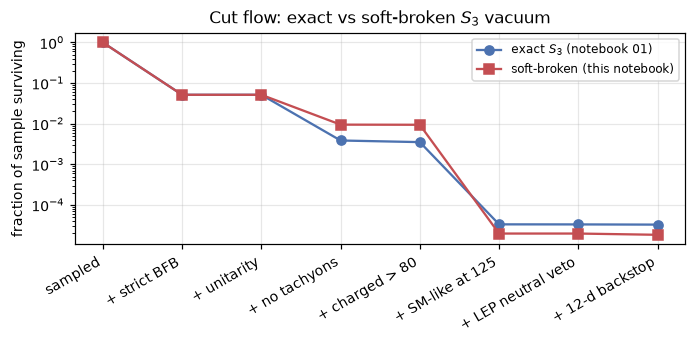
\includegraphics[width=0.78\textwidth]{figures/soft_cut_flow.png}
\caption{Cut flow, as fractions of each sample: the exact-$S_3$ scan against the soft-broken
one.}
\label{fig:cutflow}
\end{figure}

The quartic cuts remove the same 95\% in both scans, as they must. Two differences matter.
\begin{itemize}\itemsep1pt
\item \textbf{No tachyons passes 2.5$\times$ more often.} In the exact model every mass$^2$
is a quartic times $v^2$, so a $\lambda$ point with a negative combination is tachyonic for
any $\theta$. Soft terms add mass$^2$ of their own and lift those directions.
\item \textbf{The coupling cut is where the soft space dies.} The survival fraction per
sample is lower in the end, which reflects the extra prior volume as much as physics.
\end{itemize}
Chunk 0 of the cached scan is reproduced exactly by a fresh run in the notebook. Every
chunk-0 survivor's CP-even spectrum is re-derived independently from the symbolic mass
matrices.

\section{Results}
\label{sec:results}

\subsection{A decoupling-like spectrum}

\begin{center}
\begin{tabular}{lrrr@{\qquad}lrrr}
\toprule
\multicolumn{4}{c}{soft-broken [GeV]} & \multicolumn{4}{c}{exact $S_3$ [GeV]}\\
state & min & median & max & state & min & median & max\\
\midrule
$h_1$ & 34 & 125 & 128 & $H_2$ & 7 & 125 & 128\\
$h_2$ & 124 & 588 & 2419 & $h_0$ & 5 & 326 & 521\\
$h_3$ & 382 & 983 & $6\times10^4$ & $H_1$ & 122 & 370 & 849\\
$A_1$ & 55 & 595 & 2419 & $A_1$ & 2 & 333 & 671\\
$A_2$ & 304 & 990 & $6\times10^4$ & $A_2$ & 24 & 327 & 708\\
$H^\pm_1$ & 85 & 555 & 2414 & $H^\pm_1$ & 81 & 241 & 470\\
$H^\pm_2$ & 246 & 968 & $6\times10^4$ & $H^\pm_2$ & 81 & 254 & 743\\
\bottomrule
\end{tabular}
\end{center}
{\small Soft-broken states are mass-ordered within each sector. Rows are paired by role, not by
name.}

\begin{figure}[h]
\centering
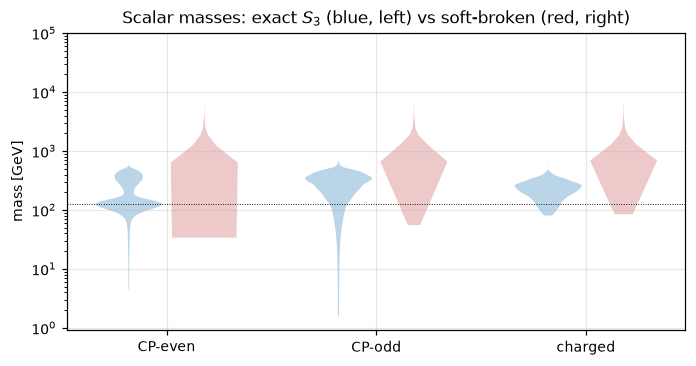
\includegraphics[width=0.78\textwidth]{figures/soft_masses.png}
\caption{Scalar masses by sector: exact $S_3$ (blue, left) against soft-broken (red, right).
The dotted line is 125~GeV.}
\label{fig:masses}
\end{figure}

In the exact scan every mass$^2$ is $\lambda\times v^2$ with $|\lambda|\le2$, so nothing
goes much beyond 850~GeV. With soft terms the heavy states are set by the soft scale. The
median heaviest scalar is 1.0~TeV, against 0.44~TeV exact, and half the points have one
above 1~TeV. The heaviest CP-even, CP-odd and charged states are near-degenerate: their
relative spread has a median of 3.7\%, and 1.5\% for $h_3>1$~TeV. That is the pattern of a
heavy doublet whose mass comes from one large soft term, the analogue of the 2HDM's
large-$m_{12}^2$ regime.

\subsection{Every state couples to $VV$, but the non-SM ones barely}

\begin{figure}[h]
\centering
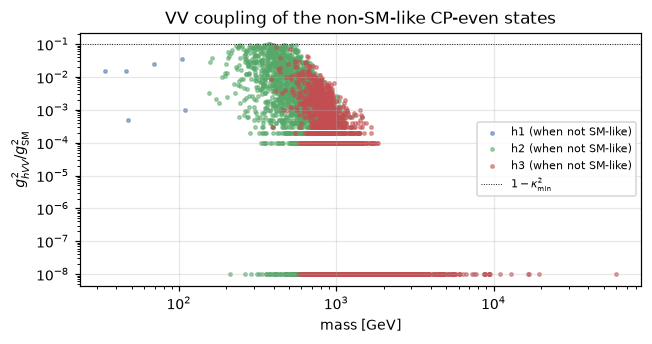
\includegraphics[width=0.76\textwidth]{figures/soft_hvv.png}
\caption{$hVV$ coupling$^2$ (in SM units) of the non-SM-like CP-even states, against their
mass. The dotted line is $1-\kappa^2_{\min}=0.1$, the most the cut allows them to carry.
The row at $10^{-8}$ collects couplings below the stored precision ($10^{-4}$, the rounding
in \texttt{viable\_points\_soft.json}), clipped onto the axis.}
\label{fig:hvv}
\end{figure}

\begin{itemize}\itemsep1pt
\item The SM-like state is $h_1$, the \emph{lightest} CP-even state, in 2015 of 2021 points
(and $h_2$ in the other 6). Its $\kappa^2$ has a median of $0.998$.
\item The other two states couple at the $10^{-4}$ level (median $4.0\times10^{-4}$, 90\%
below $1.5\times10^{-2}$, maximum $0.099$).
\item Only 6 points have a CP-even state below the SM-like one, all with $\xi^2\le0.036$,
under the LEP floor.
\end{itemize}

\subsection{The light scalars of the exact scan do not survive}

\textbf{A non-SM scalar below 100~GeV appears in 15.8\% of the exact-$S_3$ points and in
0.7\% of the soft-broken ones.} In the exact scan such states are allowed by LEP because
$h_0$ is exactly gauge-phobic and the CP-odd and charged states do not couple to $ZZ$. With
the vacuum released, no state is gauge-phobic, and generic soft breaking lifts them. The
light states are a property of the measure-zero exact slice, not of the $S_3$ quartics.
This matters for any phenomenology built on light $S_3$ scalars.

A side result: $\lambda_4>0$ holds in \emph{every} exact-scan point and in 50.6\% of the
soft-broken ones. With the alignment and $v_{1,2}>0$ fixed, the $\lambda_4<0$ aligned vacua
are all removed by the cuts. This is observed over the 1964 points, not derived.

\subsection{How much breaking do viable points need?}

\begin{figure}[h]
\centering
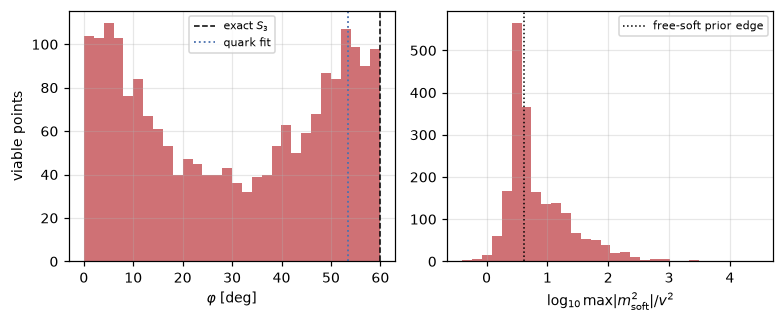
\includegraphics[width=0.86\textwidth]{figures/soft_breaking.png}
\caption{Left: survivors against $\varphi$ (uniform prior), with the exact-$S_3$ vacuum
(dashed) and the quark-fit vacuum (dotted). Right: the size of the breaking,
$\log_{10}\max|m^2_{\rm soft}|/v^2$ over all four soft terms, with the edge of the free-soft
prior.}
\label{fig:breaking}
\end{figure}

\begin{itemize}\itemsep1pt
\item \textbf{No viable point is close to exact $S_3$ in both senses at once.} The largest
soft term is at least $0.40\,v^2$, with a median of $4.1\,v^2$. Only 15 points keep every
soft term below $v^2$. Their spectra run from about 85~GeV to 630~GeV, like the exact
scan's heavy states but without its very light ones. Some of this is the prior, since a
uniform box in $m^2$ gives little volume to small values. What the scan does show is that
small breaking is \emph{allowed}, including within a few degrees of $60^\circ$, and that the
viable region does not collapse onto the exact vacuum. It only becomes rare under this
measure.
\item \textbf{Survivors pile up at both ends of the domain} (261 in the first $5^\circ$,
237 in the last, about 95 per bin in the middle). The $\varphi\to0$ end is the decoupling
tail: the solved $m_{D1}^2\propto1/(v_1v_2)$ blows up there, and all 34 points with a state
above 5~TeV have $\varphi<7^\circ$ (Fig.~\ref{fig:mD1}). The $\varphi\to60^\circ$ end has
moderate breaking (median $3.5\,v^2$ within $10^\circ$).
\item \textbf{The quark-fit vacuum is well populated}: 205 points lie within $\pm2^\circ$ of
$\varphi=53.4^\circ$.
\end{itemize}

\begin{figure}[h]
\centering
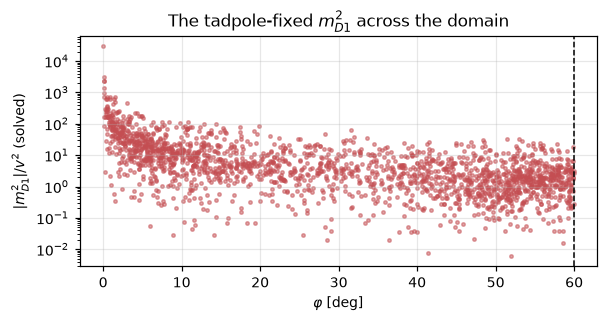
\includegraphics[width=0.66\textwidth]{figures/soft_mD1_edge.png}
\caption{The tadpole-fixed $|m_{D1}^2|/v^2$ across the domain. It grows without bound as
$\varphi\to0$, which is where the multi-TeV tail comes from.}
\label{fig:mD1}
\end{figure}

\clearpage
\section{Open questions, and what would help}

\begin{enumerate}\itemsep4pt
\item \textbf{The near-$S_3$ corner.} A uniform prior in $m^2$ leaves only 15 points with
every soft term below $v^2$. Whether the light gauge-phobic scalars reappear continuously as
the breaking shrinks needs a targeted scan, with log-uniform soft terms and $\varphi$ near
$\pi/3$.
\item \textbf{Global minimum.} The scan requires only a local minimum. With soft terms the
potential can have several minima, so a multi-start minimisation on the survivors is the
missing vacuum-stability cut.
\item \textbf{Decays and LFV on the soft points.} The decays analysis parametrises the
CP-even sector by one angle $\delta$, which assumes the aligned $2\times2$ block. The soft
points carry a full $3\times3$ mixing matrix (stored per point), so the couplings and rates
have to be regenerated. This is also where the quark channels can finally enter, since the
soft-broken quark sector works.
\item \textbf{Which vacuum do we want to present?} The quark fit picks a region of the domain
that is well populated here. Is the combined statement worth making in the LFV paper: a
soft-broken vacuum that reproduces CKM magnitudes, passes the scalar cuts, and has a
decoupling-like spectrum? Your call.
\end{enumerate}

\appendix
\section{The derivation ledger}

The full typeset version is the companion document \texttt{derivations\_05.tex}; in
summary:

\begin{center}
\begin{tabular}{p{0.30\textwidth}p{0.13\textwidth}p{0.47\textwidth}}
\toprule
claim & status & independent checks\\
\midrule
The tadpoles fix $(\mu_0^2,\mu_1^2,m_{D1}^2)$ for a general vacuum & derived &
solving for $m_{D2}^2$ instead is singular at $\varphi=45^\circ$; $m_{D1}^2=0$ on the aligned,
zero-soft vacuum\\
\addlinespace
Goldstones isolated; CP-even $3\times3$ with no gauge-phobic state & derived &
exact zeros at a rational point; 30-digit brute force at 60 points; sum rule to $10^{-15}$\\
\addlinespace
$\varphi\in(0,\pi/3)$ is a fundamental domain & derived &
identical spectra at 200 image pairs; fails if the $\mathbf2$ spurion is left untransformed\\
\addlinespace
$r=-\cot(\varphi-\pi/6)$ & derived &
agrees with the verified basis map at 40 angles; $|r(\pi/3)|=\sqrt3$\\
\addlinespace
Soft terms need not be small & \textbf{imported} \cite{tHooft80} &
technical naturalness\\
\bottomrule
\end{tabular}
\end{center}

\begin{thebibliography}{9}

\bibitem{tHooft80} G.~'t~Hooft,
\emph{Naturalness, chiral symmetry, and spontaneous chiral symmetry breaking},
NATO Sci.\ Ser.\ B \textbf{59}, 135 (1980),
\href{https://doi.org/10.1007/978-1-4684-7571-5_9}{doi:10.1007/978-1-4684-7571-5\_9}.

\bibitem{GomezBock21} M.~Gómez-Bock, M.~Mondragón and A.~Pérez-Martínez,
\emph{Scalar and gauge sectors in the 3-Higgs Doublet Model under the $S_3$-symmetry},
Eur.\ Phys.\ J.\ C \textbf{81}, 942 (2021),
\href{https://arxiv.org/abs/2102.02800}{arXiv:2102.02800},
\href{https://doi.org/10.1140/epjc/s10052-021-09731-3}{doi:10.1140/epjc/s10052-021-09731-3}.

\end{thebibliography}

\end{document}
